

\section{Experiments}
\label{experiment}

According to the work done by \citeauthor{Hachemi:2011jn} \cite{Hachemi:2011jn}, a tensile experiment is carried on a universal traction machine, to figure out whether the braid angle decrease consistents with the model they proposed.



%% how the experiment is done
%%% condition


\begin{figure}[!htbp]
    \centering
    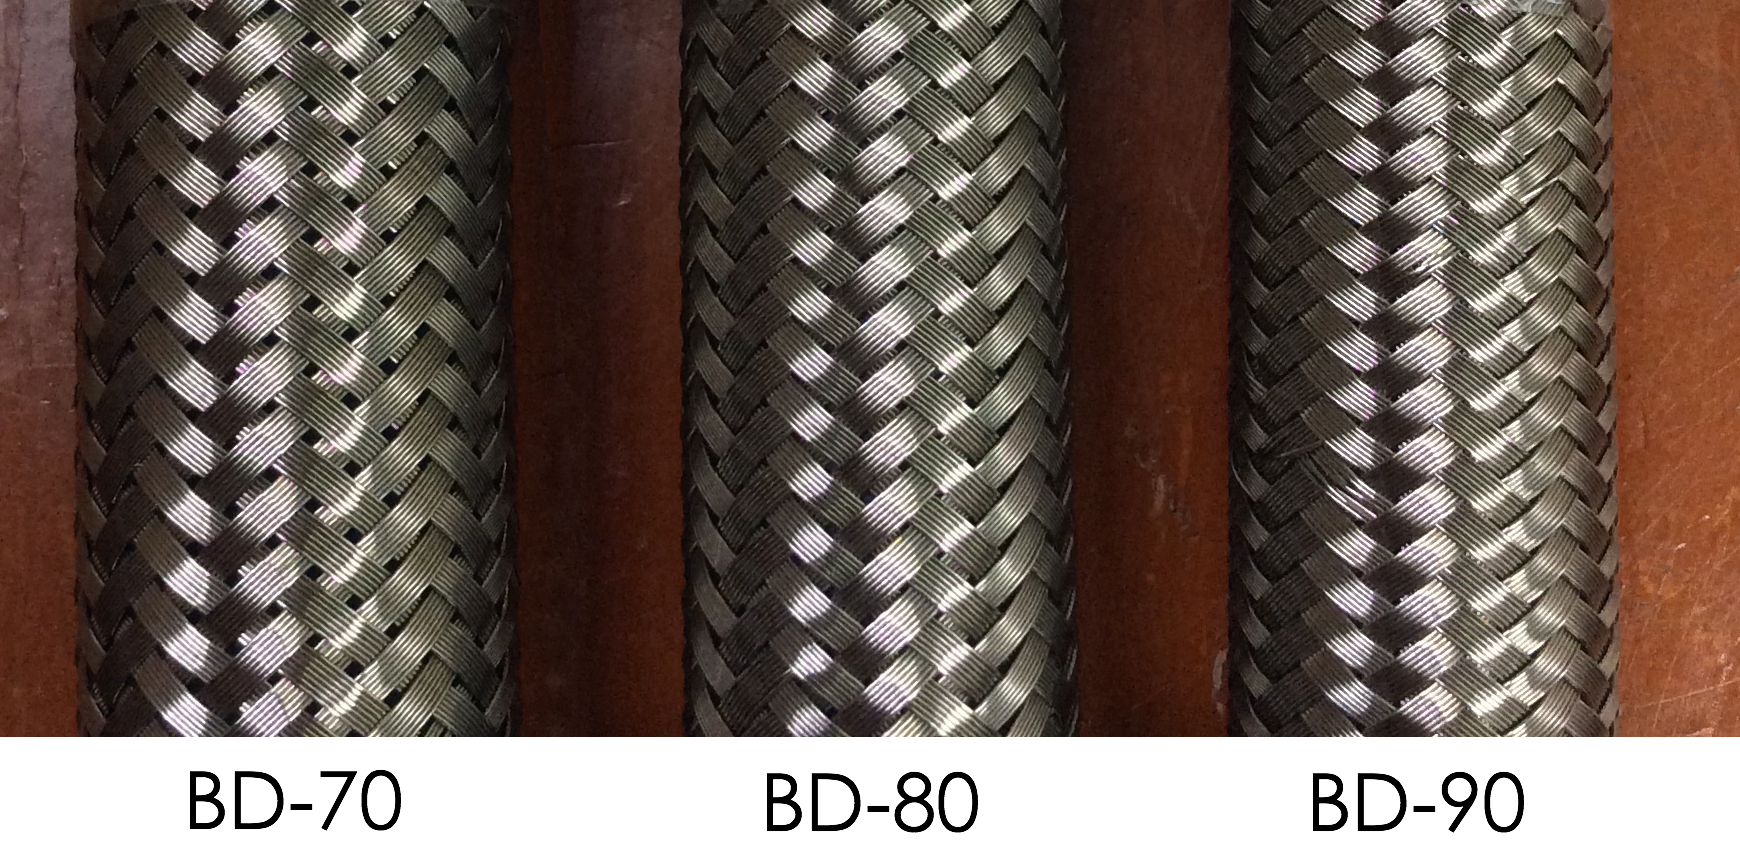
\includegraphics[width=0.8\linewidth]{figure/experiment/18mm-hose-specimen}
    \caption{}
    \label{fig:18mm-hose-specimen}
\end{figure}



%%% data operation
\begin{figure}
    \centering
    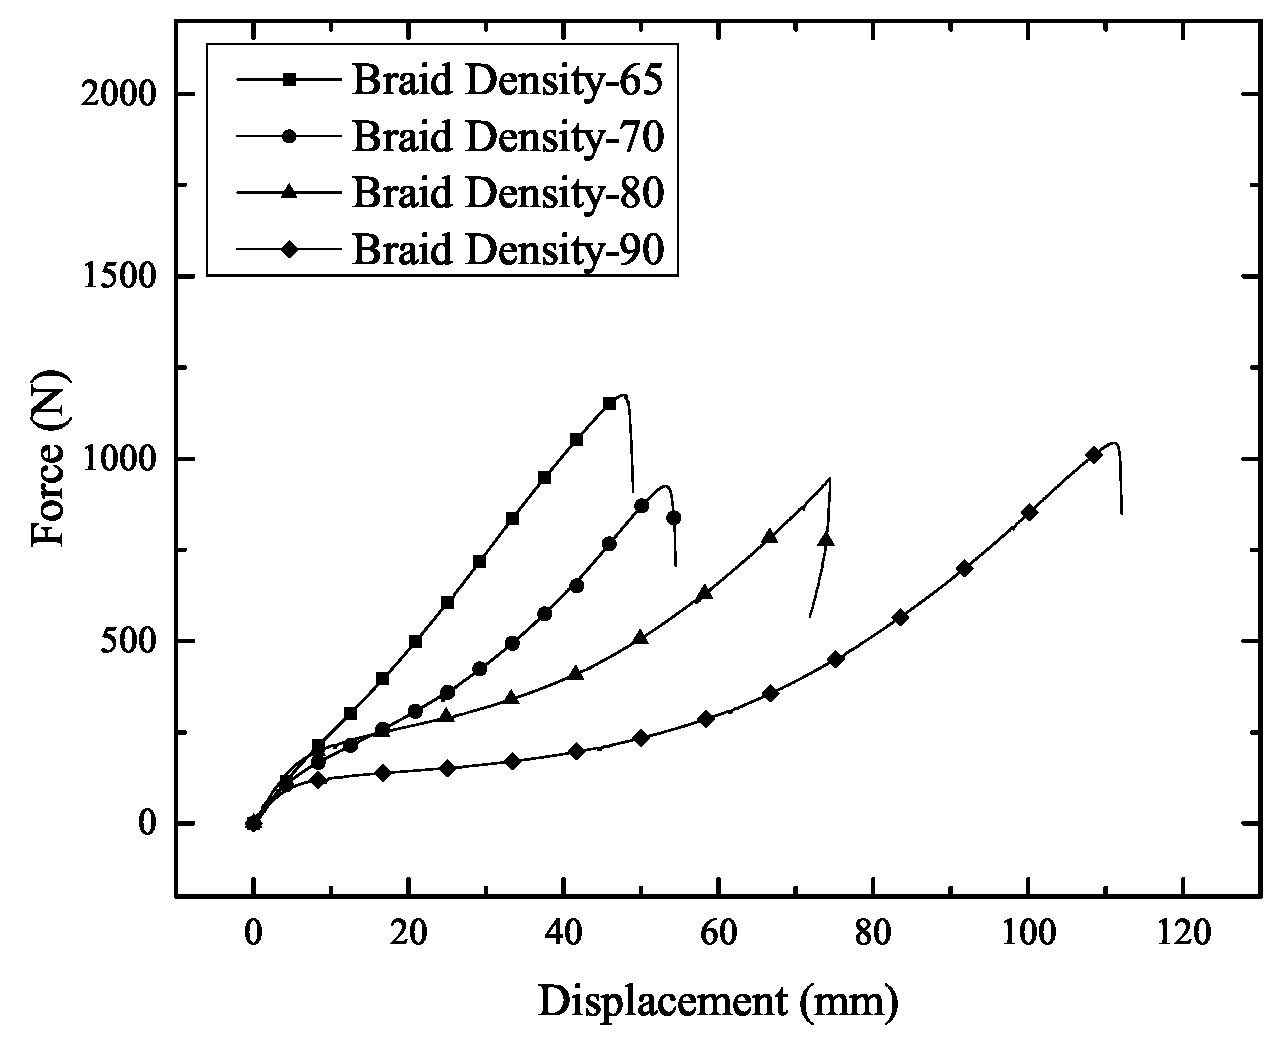
\includegraphics[width=0.7\linewidth]{figure/experiment/E3-G4/Graph01}
    \caption{}
    \label{fig:graph01}
\end{figure}


%% experiment results

%% CAE results comparation




